\section{Privacy Protection against Real-World Apps}
\label{sec:protecting_up}

In Figure~\ref{fig:intro_case_study_uber}, we showed how \framework{} can be effectively used to protect user privacy while they are using Uber. In this section, we use three more real-world Android apps to showcase privacy advantages of \framework{}.

\subsection{com.katana.facebook (v404.0.0.35.70)}
\label{sec:fb_case_study}
 
During the experiment, while scrolling through Facebook’s \textit{Home} activity without engaging other features, \framework{}'s \textit{Resource Access Log Reporter} detected unexpected microphone access, as shown in Figure~\ref{fig:case-study-facebook}a. Further investigation revealed that Facebook was using \texttt{MediaRecorder} to access the device microphone. Surprisingly, Android’s privacy indicator~\cite{andPrivacyIndicator} (green dot), which signals active microphone use, did not appear when \framework{} logged the access.

To verify this, we created a custom app that used the \texttt{MediaRecorder} API to record audio, and the privacy indicator remained absent, confirming a likely bug in its implementation. We have reported this issue to Android and plan to responsibly open-source our test app.

\framework{} not only detected this hidden microphone usage but also successfully spoofed the requested audio data, ensuring user privacy.

Similarly, \framework{} logged instances of Facebook accessing calendar data while searching for nearby events. The app reads user calendar events to determine availability when displaying event suggestions. User can configure \framework{} to manipulate calendar data, allowing Facebook to receive general availability details while concealing sensitive event information by spoofing fields like event names and locations.

\begin{figure}[t]
    \centering
    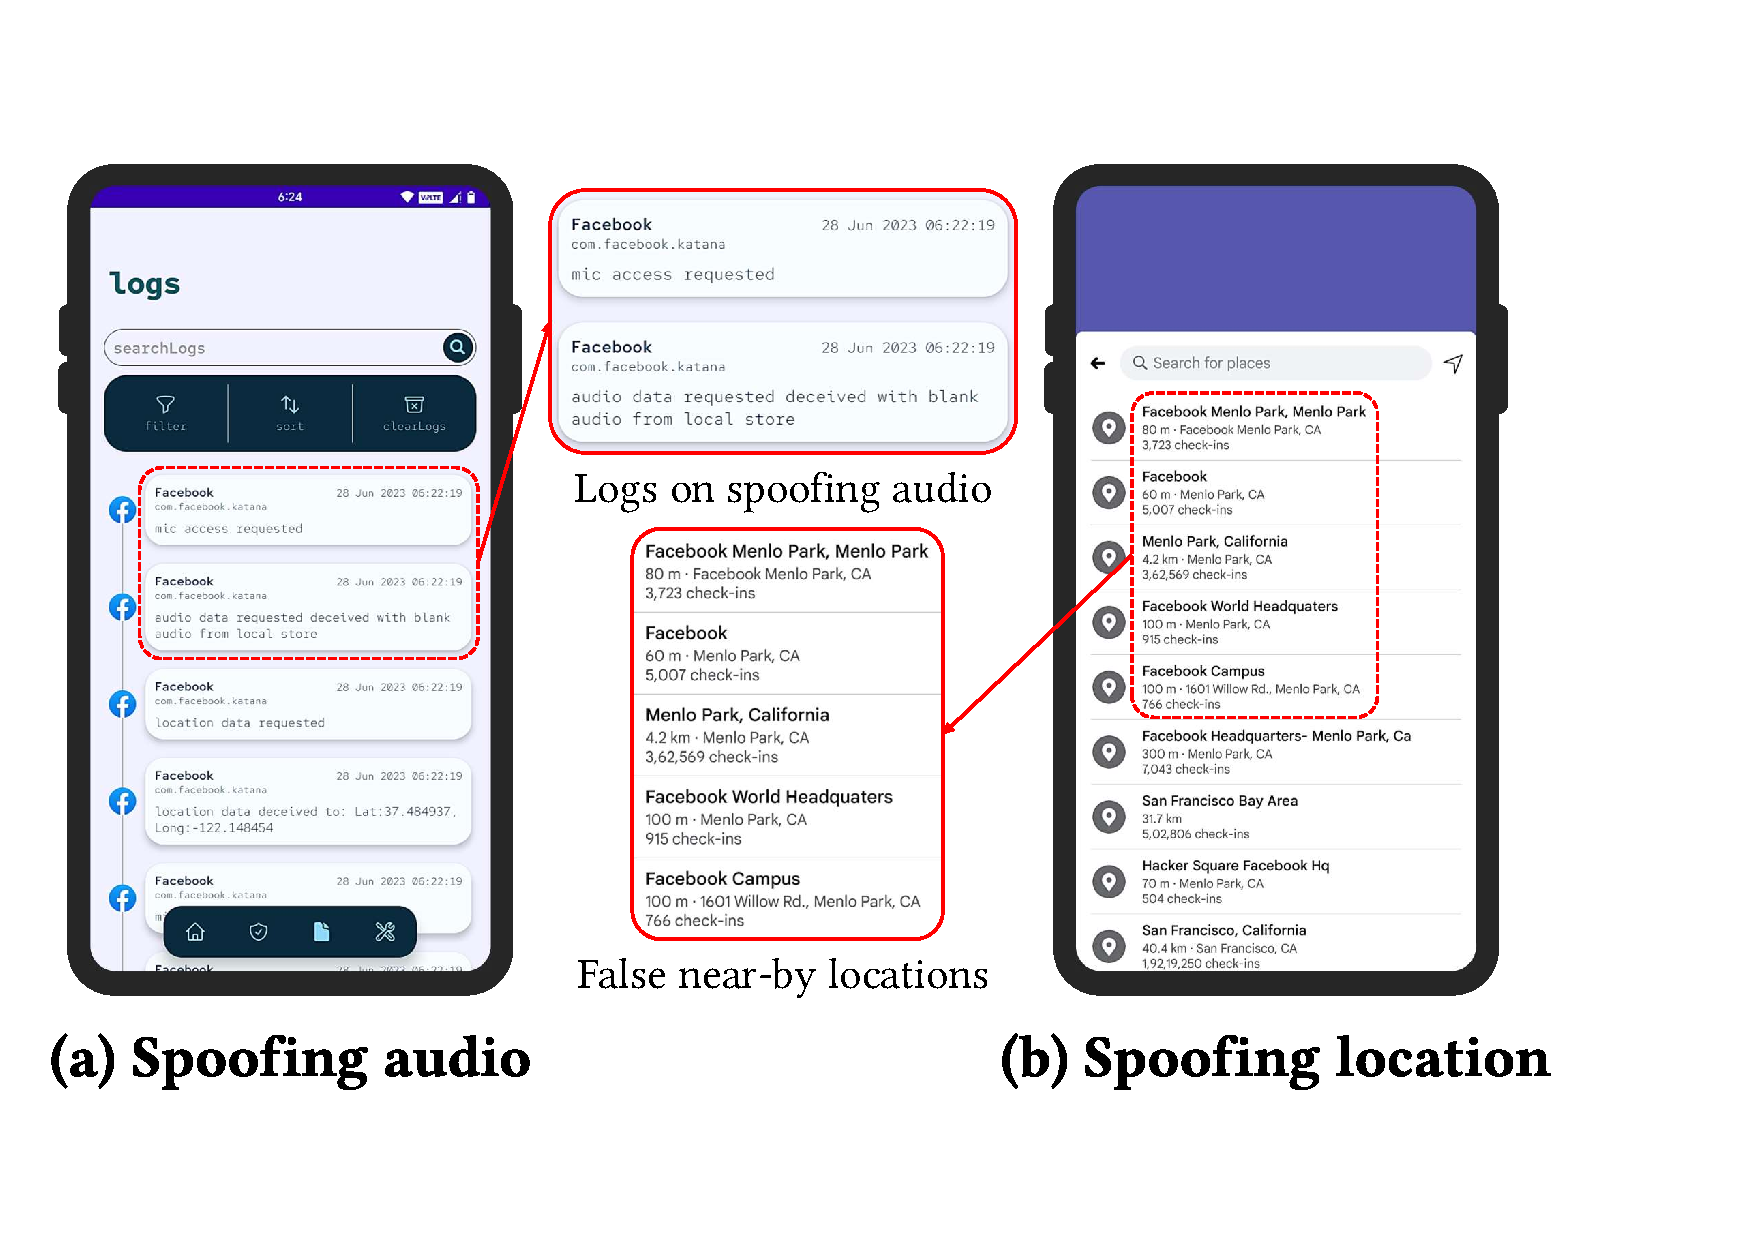
\includegraphics[width=0.75\linewidth]{Figures/Case Studies/facebook_screenshots.pdf}
    \caption{Screenshots demonstrating deceiving location and audio data using \framework{} for the Facebook app.}
    \label{fig:case-study-facebook}
\end{figure}

Additionally, as shown in Figure~\ref{fig:case-study-facebook}b, \framework{} effectively spoofed fine-grained GPS location data with a nearby location. This ensured that Facebook could still display relevant nearby places and events without revealing the user’s exact location.

\subsection{com.snapchat.android (v12.24.0.34)}
\label{sec:sc_case_study}

\begin{figure}[t]
    \centering
    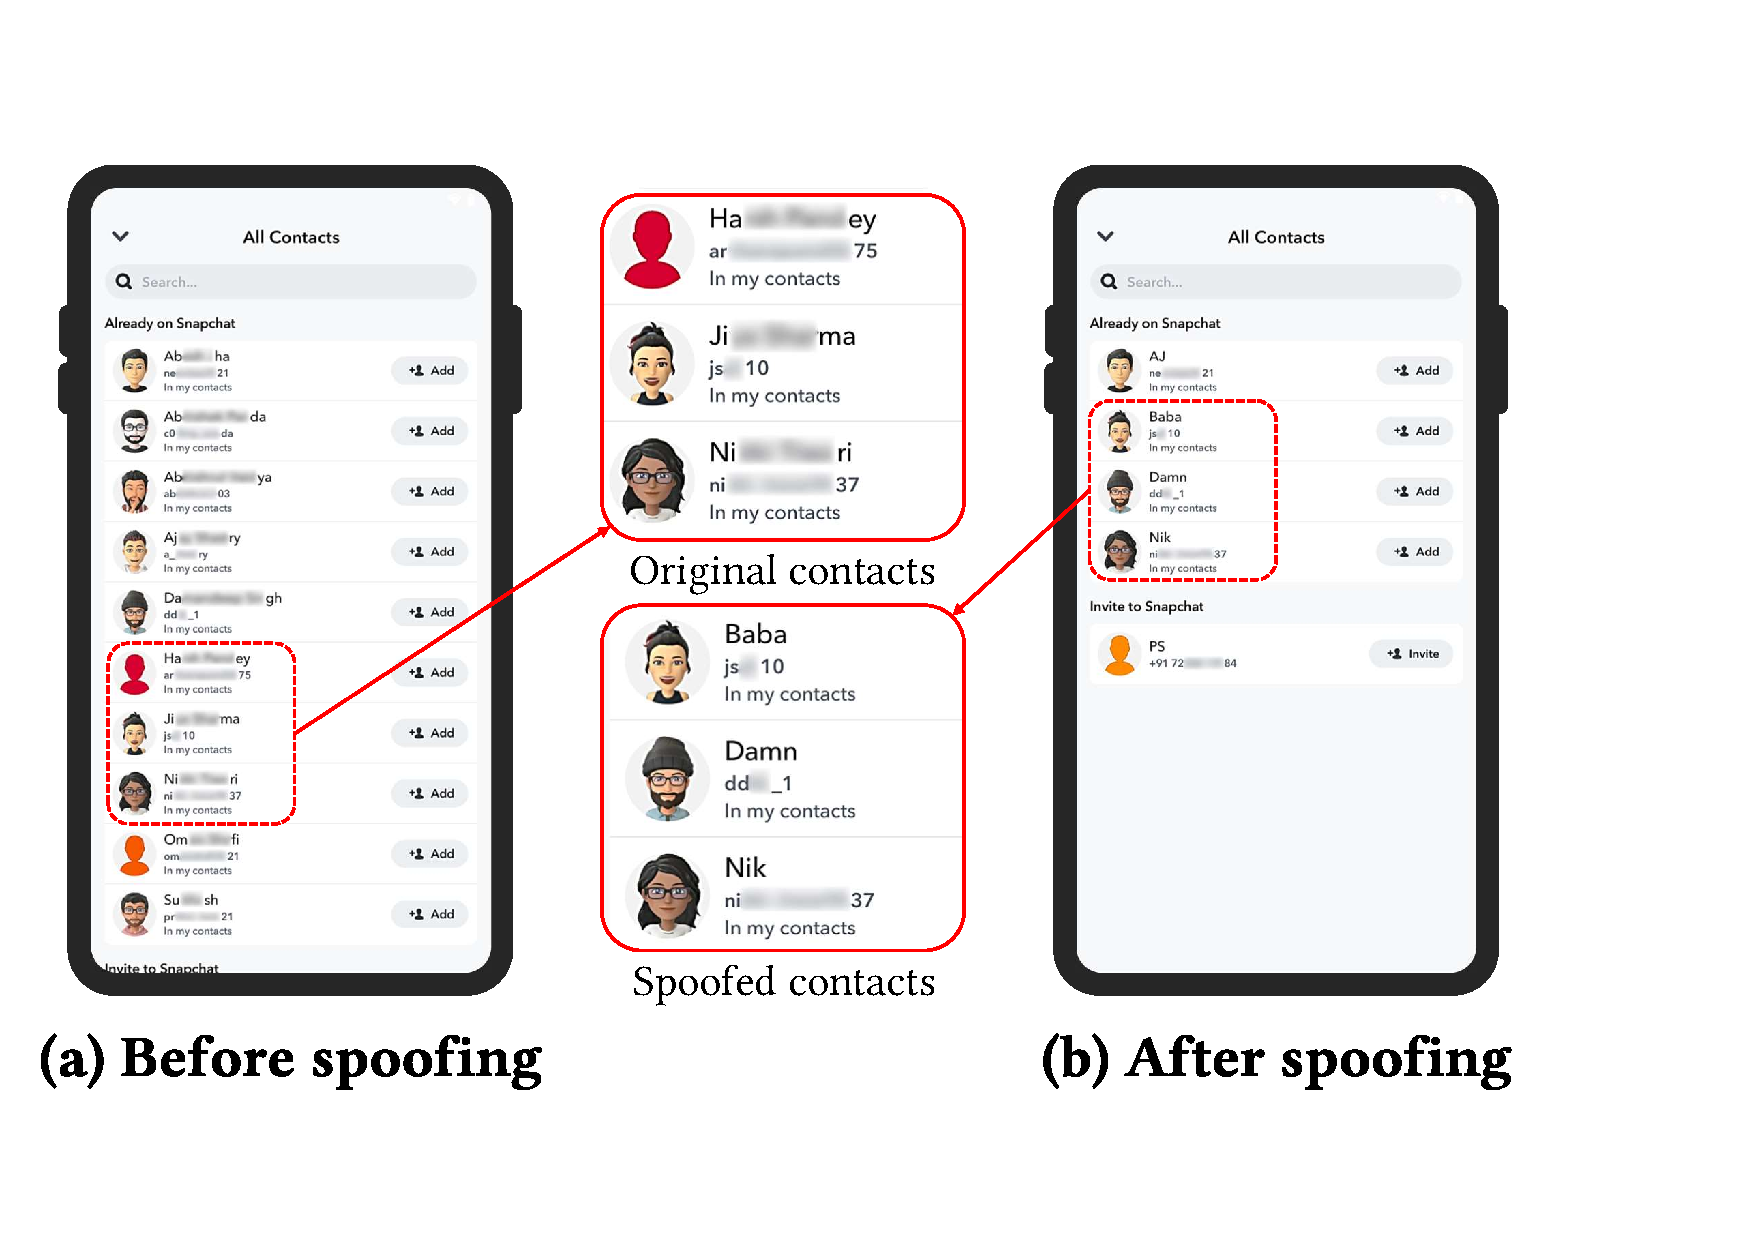
\includegraphics[width=0.75\linewidth]{Figures/Case Studies/snapchat_screenshots.pdf}
    \caption{Screenshots demonstrating how user can share spoofed contacts using WhiteLie with Snapchat.}
    \label{fig:case-study-snapchat}
\end{figure}

Snapchat's \textit{Snap Map} feature uses GPS and sensor data to display user avatars and real-time activities. While \textit{Ghost Mode} prevents location sharing, it disables \textit{Snap Map} features and does not ensure that the app isn't still accessing location data.

\framework{} effectively spoofed GPS location and \texttt{READ\_CONTACTS} permissions using predefined contact lists in its \textit{Deceit} section, as shown in Figure~\ref{fig:case-study-snapchat}b. This allows users to control the data they share with Snapchat while still accessing \textit{Snap Map} features.

\subsection{com.truecaller (v12.54.7)}
\label{sec:tc_case_study}
Truecaller identifies spam messages by analyzing incoming texts but requires access to all user messages. \framework{} successfully spoofed message content while preserving the sender's phone number. This allows users to maintain message privacy while still benefiting from spam detection, as shown in Figure~\ref{fig:case-study-truecaller}b.

\begin{figure}
    \centering
    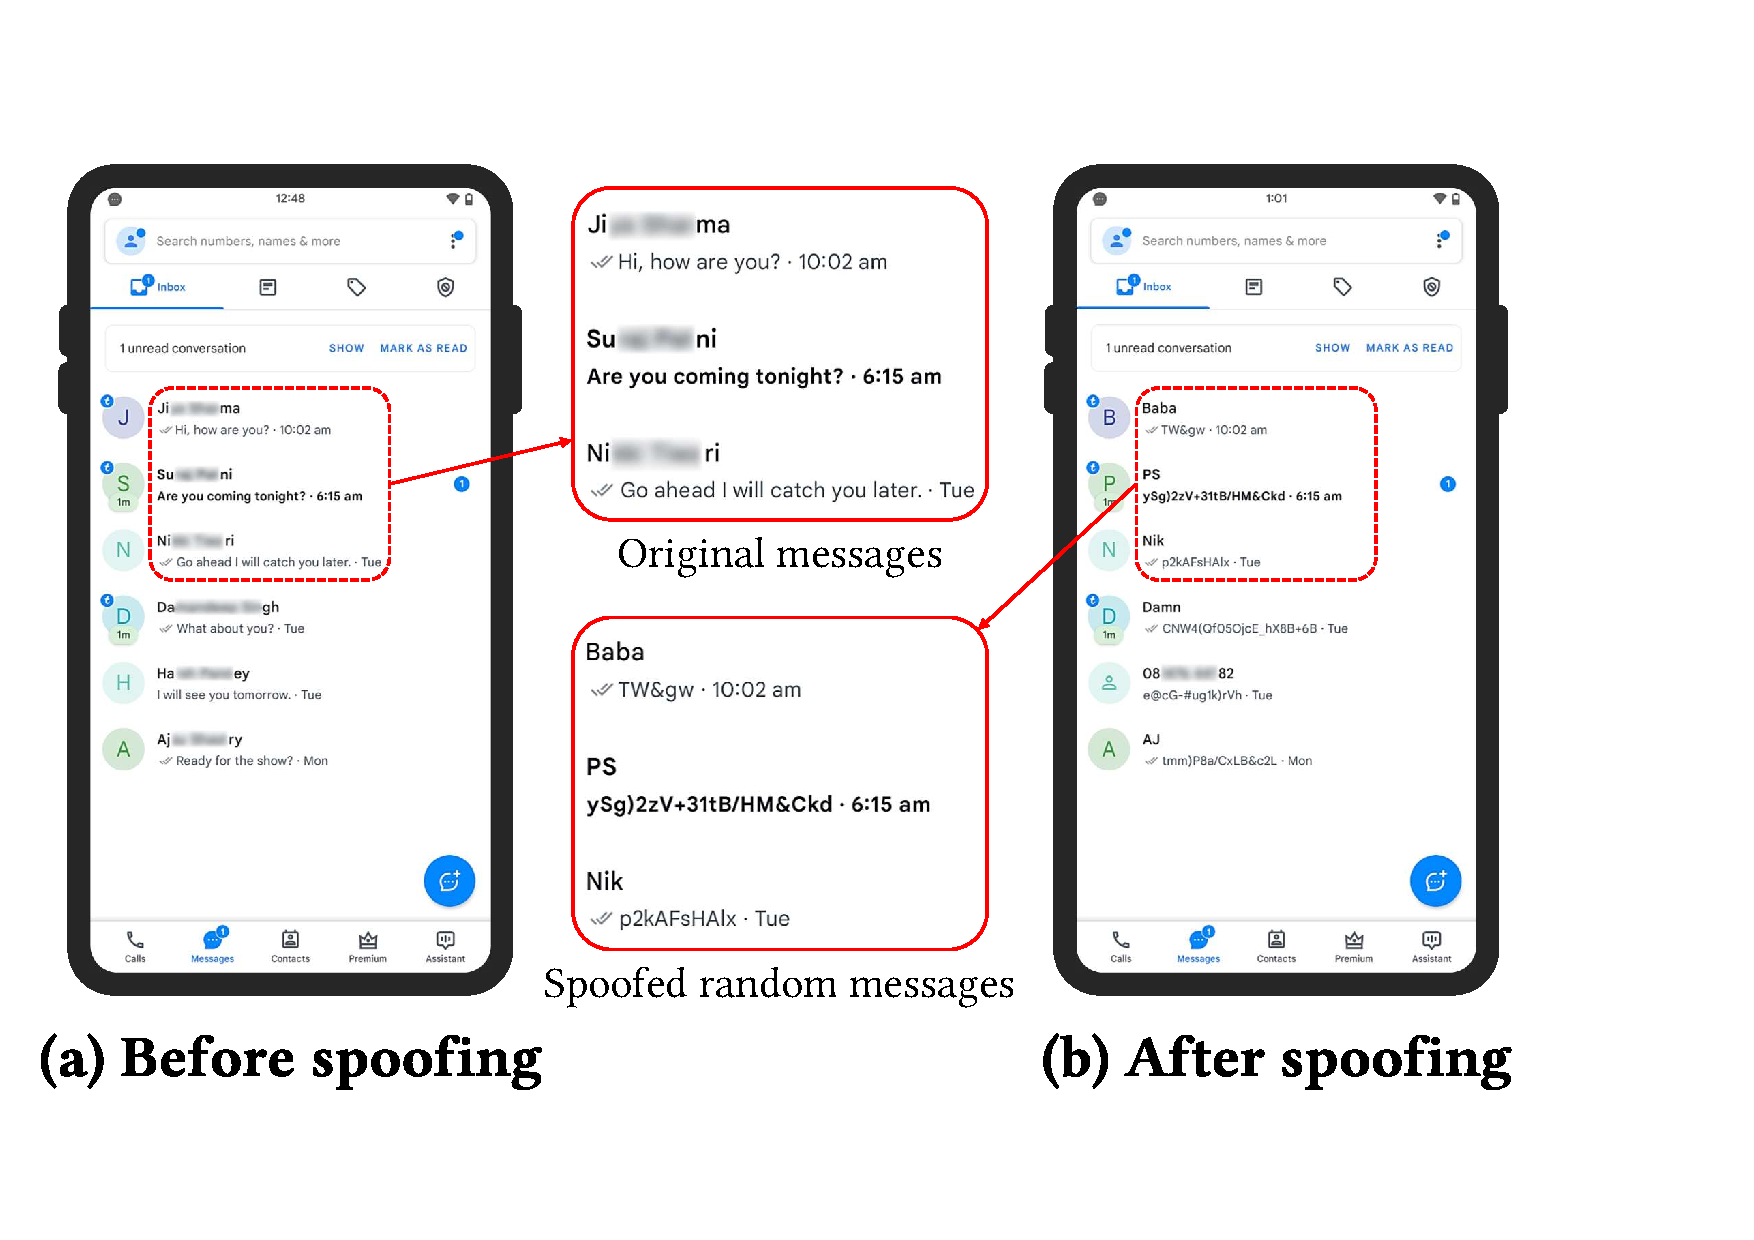
\includegraphics[width=0.75\linewidth]{Figures/Case Studies/truecaller_screenshots.pdf}
    \caption{Screenshots demonstrating how a user can share spoofed SMS using WhiteLie with Truecaller app.}
    \label{fig:case-study-truecaller}
\end{figure}

\textit{Overall, this section shows that \framework{} empowers users to fully use the app features while controlling the information that they share with the apps.}
